\documentclass[12pt, letterpaper]{report}
\usepackage[nonumberlist, toc]{glossaries}
\usepackage{listings}
\usepackage{graphicx}
\graphicspath{ {graphics/} }
\makeglossaries
%\definecolor{mymauve}{rgb}{0.58,0,0.82}
\lstdefinelanguage{JavaScript}
{
  keywords={typeof, new, true, false, catch, function, return, 		null, catch, switch, var, if, in, while, do, else, case, break, require},
  comment=[s]{/*}{*/},
  morecomment=[l]//,
  string=[b]",
  morestring=[b]'
}

%%%%%%%%%%%%%%%%%%%%%%%%%%%%%%%%%%%%%%%%%%%%%%%%%%%%%%%%%%%%%%%%%%%%%%%%
%	All glossary entries are defined here.  These must be compiled
%	outside of Gummi and will show in the final document.
%
%	Commands
%		$latex report
%		$makeglossaries report
%		$latex report
%
%	This produces a div file which can be converted to a pdf
%%%%%%%%%%%%%%%%%%%%%%%%%%%%%%%%%%%%%%%%%%%%%%%%%%%%%%%%%%%%%%%%%%%%%%%%

\newglossaryentry{MOO}
{
	name={MOO},
	description={MUD (Multi-User Domain), Object Oriented. a text-based online virtual reality system to which multiple users (players) are connected at the same time.}
}
\newglossaryentry{MUD}
{
	name={MUD},
	description={Multi-User Domain. A multiplayer real-time virtual world, usually text-based. MUDs combine elements of role-playing games, hack and slash, player versus player, interactive fiction, and online chat.}
}
\newglossaryentry{LambdaMOO}
{
	name={LambdaMOO Server},
	description={A network-accessible, multi-user, programmable, interactive system well-suited to the construction of text-based adventure games, conferencing systems, and other collaborative software}
}
\newglossaryentry{enCore}
{
	name={enCore},
	description={A computer program that allows multiple users to connect via the Internet to a shared database of rooms and other objects and interact with each other and the database in real time}
}
\newglossaryentry{TECFAMOO}
{
	name={TECFAMOO},
	description={A text-based virtual reality. It is a Virtual Space for Educational Technology, Education, Research and Life at TECFA, School of Psychology and Education, University of Geneva, Switzerland}
}
\newglossaryentry{TKMOO}
{
	name={TKMOO},
	description={An advanced chat client suitable for use with MUDs and especially MOO systems.}
}
\newglossaryentry{MOOtcan}
{
	name={MOOtcan},
	description={A simple MOO-client, Java applet, used in enCore. It is currently only usable for MOO-connections as it sends and read lines, not characters, through and from the socket. This class glues together a GUI (currently only a panel inside a frame) and a network-connection. It supports processing of the stream from the MOO.}
}
\newglossaryentry{XP}
{
	name={eXtreme Programming},
	description={An incremental software development methodology that stresses communication, estimation, planning, testing, flexibility, and other practices. It is associated with other methodologies that implement agile development}
}
\newglossaryentry{freeSoftware}
{
	name={Free Software},
	description={Software licensed such that the user has the freedom to run, redistribute, and study the source code as they wish}
}
\newglossaryentry{LARP}
{
	name={Live Action Role Play},
	description={A role playing game where players physically act as their characters, inspired by similar tabletop games}
}
\newglossaryentry{GNU}
{
    name={GNU},
    description={A free software operating system developed by the GNU project. Its software is typically bundled with the Linux kernel to form an operating system commonly called Linux. GNU is a recursive acronym, standing for 'GNU's Not Unix!'}
}
\glsaddall

%%%%%%%%%%%%%%%%%%%%%%%%%%%%%%%%%%%%%%%%%%%%%%%%%%%%%%%%%%%%%%%%%%%%%%%%
%	All the title page information is listed here
%%%%%%%%%%%%%%%%%%%%%%%%%%%%%%%%%%%%%%%%%%%%%%%%%%%%%%%%%%%%%%%%%%%%%%%%

\author{Owen Watson, John Lewis, Tim Cunningham}
\title{Literary Worlds Project Report}
\date{March 12, 2014}
\linespread{1.25}


\usepackage{graphicx}
\begin{document}
%%%%%%%%%%%%%%%%%%%%%%%%%%%%%%%%%%%%%%%%%%%%%%%%%%%%%%%%%%%%%%%%%%%%%%%%
%	Title Page
%%%%%%%%%%%%%%%%%%%%%%%%%%%%%%%%%%%%%%%%%%%%%%%%%%%%%%%%%%%%%%%%%%%%%%%%
\begin{titlepage}
\Huge \maketitle \par
\end{titlepage}

%%%%%%%%%%%%%%%%%%%%%%%%%%%%%%%%%%%%%%%%%%%%%%%%%%%%%%%%%%%%%%%%%%%%%%%%
%	Abstract
%
%	May need to be changed to reflect what is written later.
%%%%%%%%%%%%%%%%%%%%%%%%%%%%%%%%%%%%%%%%%%%%%%%%%%%%%%%%%%%%%%%%%%%%%%%%

\chapter{Abstract}
\par
EnCore Literary Worlds is an interactive, networked environment for exploration of literary works. Each environment is created by an ordinary user familiar with the source work, to create a more immersive experience for other users and students. The system is designed to be very easy for new and non-technical users, as well as being complex enough for creation of manipulable objects, abilities, and interaction between users in the environment.

\par
The EnCore Literary Worlds system can be used for many genres and types of worlds, with both original or derivative works. It can be used to extrapolate source text, create second worlds, create role play or alternative reality, or even virtual tours and museums. This is explained by Allen Webb,

%-- page 4 - Teaching Literature in Virtual Worlds --%
\begin{quotation}
While all of the literary virtual worlds described in this book [Teaching Literature in Virtual Worlds] allow group interaction, several are explicitly designed as Alternative Reality Games (ARG) activities (%
\textit{Thoughtcrime, Midsummer Madness, The Virtual Tempest}). Other worlds (%
\textit{The Village of Umufofia, Mice, Men, and Migrant Labor, Gatsby's American Dream})
could be described as a virtual Live Action Role Plays (LARPs), activities typically prepared by a "gamemaster", in this case the virtual world builder.\cite[4]{Webb}
\end{quotation}

\par
This project proposes a drop in replacement for the first software release for the existing, outdated Java browser applet for interacting with the EnCore Literary Worlds system. The new system will be fully compatible with the existing script, server and backend tools and will work with common web browsers, both on desktop and mobile platforms well into the future, being built with JavaScript and other current web technologies.



\par
Further releases may augment the feature set offered by the browser client, update the version of the enCore software, or implement other client stories as needed.

%%%%%%%%%%%%%%%%%%%%%%%%%%%%%%%%%%%%%%%%%%%%%%%%%%%%%%%%%%%%%%%%%%%%%%%%
%	Table of Contents 
%%%%%%%%%%%%%%%%%%%%%%%%%%%%%%%%%%%%%%%%%%%%%%%%%%%%%%%%%%%%%%%%%%%%%%%%
	
\tableofcontents

%%%%%%%%%%%%%%%%%%%%%%%%%%%%%%%%%%%%%%%%%%%%%%%%%%%%%%%%%%%%%%%%%%%%%%%%
%	Start of Background Chapter.
%
%	The background chapter will contain the following:
%		Client Introduction
%			-The who, what, when, and where of the original project
%			-What is the project
%			-Any and everything else about the client
%		Current Events on the Literate Worlds Project
%			-Current status of the project
%			-Problems
%			-Solution to this problem
%		Our Solution to the problem
%			-What is our solution
%			-Describe how this solves the problems
%			-What can be done in the future
%%%%%%%%%%%%%%%%%%%%%%%%%%%%%%%%%%%%%%%%%%%%%%%%%%%%%%%%%%%%%%%%%%%%%%%%

%-- Index --%
\chapter{Background}

\section{The People Behind Literary Worlds}
\par
Allen Webb is a professor of Comparative Literature and Postcolonial Studies in the Western Michigan University Department of English. He edited the book, \textit{Teaching Literature in Virtual Worlds} (among other books, articles and presentations), and designed a literary virtual world (Village of Umuofia) for which he was awarded the A+ Award by Web English Teacher.

\par
Robert Rozema is a professor of English Education at Grand Valley State University.  In the processes of completing a doctoral degree, he built (along with his students) the prototype virtual literary world, while studying Aldous Huxley's \textit{Brave New World}. Robert was awarded the National Technology Leadership Award for his experience and use of the literary world for education.  He completed his doctoral degree under Dr. Allen Web in 2004.

\par
The initial literary world created by Robert, along with several others created by Joe Haughey (doctoral student in English Education at Western Michigan University), Cara Aver (graduate student in Arts of Teaching English at Western Michigan University) and Allen Web, became the foundation for the grant that funded the Literary Worlds project.\cite{VirtWorldsTech}

\section{Funding}
\par
Funding for the Literary Worlds projects came from the President's Innovation Fund.  The past president of Western Michigan University, Judtih I. Bailey, created the grant, looking for "truly transformational" ideas. A pool of \$2 million was to be distributed to selected projects, ranging from \$25,000 to \$1 million. Literary Worlds was one of seven project select to receive money from this grant. \$116,898 was awarded to the Literary Worlds project.\cite{VirtWorldsTech}

\section{Technology}
\par
\textit{Virtual Worlds for Literary Study: Technological Pedagogical Content Knowledge in \textit{The Village of Umuofia} and other Literary Worlds} describes the technology stack employed by the Literary Worlds project:
\begin{quotation}
The technology framework for the Literary Worlds Project is enCore 4, an free software software package emerging from text-based multi-user domain technology and designed for educational use. Built on LambdaMOO (a Multi-user domain Object Oriented, created in January 1991 by Pavel Curtis at Xerox PARC.\cite{Wired}) with a built-in server-side client called Xpress, enCore allows builders to create online learning environments, featuring visual images, easy navigation between rooms, static avatars, synchronous participant communication, textual activities, the incorporation and complex utilization of a wide range of objects including textual, visual, audio and video files, maintenance of running records of actions and speech, the incorporation of bots (virtual characters with a pre-programmed speaking repertoire), and a wide range of programmable options.  EnCore is not three dimensional, but it is an immersive, self-contained multi-user virtual environment (MUVE).\cite{VirtWorldsTech}
\end{quotation}
\par 
The enCore MOO project was created in 1997, its aim to to create easy and convenient access to MOO systems and scripts by creating a point and click interface around the typically text based existing tools. EnCore is based on the Feb 02, 1997 version of the original LambdaCore Database and supplemented with a number of useful educational tools and enhancements, such as support for the enCore Xpress and MacMOOSE interfaces. Literary Worlds uses enCore version 4 to allow users access to the created virtual worlds.

\par
The existing system uses the enCore Xpress Java browser applet on the client end. The server end of the system runs on Mac OS X, version 10.6.8, with two 2.66 gigahertz dual core Xeon processors, four gigabytes of RAM, and several hard disks. A replacement system would likely be deployed on CentOS, Ubuntu or Debian Linux since there is no licensing fee or special hardware requirement.

\par
\begin{figure}[ht!]
\centering
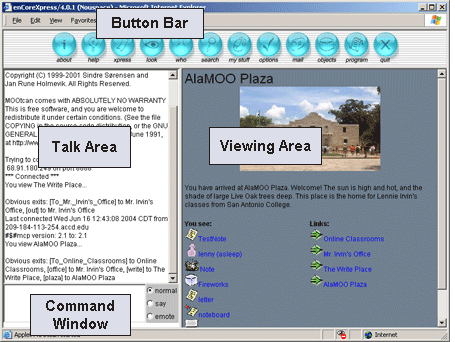
\includegraphics{enCoreScreen.png}
\caption{A screenshot of the existing enCore Xpress system}
\label{overflow}
\end{figure}

%%%%%%%%%%%%%%%%%%%%%%%%%%%%%%%%%%%%%%%%%%%%%%%%%%%%%%%%%%%%%%%%%%%%%%%%
%	Start of Stories Chapter
%
%	The stories chapter will contain the following:
%		-An explanation of stories in XP
%		-Explain the projects functionality and requirements
%		-A general explanation of each story for the project
%		-Total time and risk for release one 
%%%%%%%%%%%%%%%%%%%%%%%%%%%%%%%%%%%%%%%%%%%%%%%%%%%%%%%%%%%%%%%%%%%%%%%
\chapter{Stories}
\par
In eXtreme Programming, stories are functional descriptions in the system. The stories are rigorously defined such that there is no doubt whether or not the story is implemented correctly and completely. The stories will be written, a short description of the functionality in question. Then, the story will be estimated by the development team. Upon this feedback, the client is able to prioritize which stories get implemented first so that each release contains the most important functions.

\par
As it stands now, the statement made in "Teaching Literature in Virtual Worlds", that 

\begin{quotation}
All is needed [to access Literary Worlds] is web access and a standard browser set to 'accept popups'(Webb 9)
\end{quotation}
is no longer true. Java browser applets have fallen out of favor, and therefore require significant configuration on the user end to access Literary Worlds. Moving into the future, fewer and fewer users will have Java applets enabled on their desktop computers, and none of the major mobile platforms currently support a Java Runtime Environment in the browser. Therefore, a new client compatible with current and future browsers is needed.

\par
The new system will provide a secure, convenient interface to the existing system, over the telnet networking protocol. The first release of the system will strictly a feature for feature reimplementation of the Java browser applet system, using JavaScript and Node.js. This will ensure that Literary Worlds can be used by school districts, literary enthusiasts, and the general public without time consuming and potentially insecure modifications to their web browser configuration. It will also ensure that the system will be accessible through new web platforms, on smart phones and tablets of all types and operating systems.

\section{Console Interface}
The most basic implementation of the software will provide the text console interface that of original Java applet. This input will be accepted in a console interface, and will then be sent back to the telnet server running under EnCore v4, and the console response sent back to the user's terminal.

\section{Graphical Interface}
The secondary functionality of the original Java applet is the graphical interface, which displays text, images, video, audio, and other multimedia. This interface provides a more intuitive and less intimidating way for users to interact with the literary worlds. 

\section{Secondary Features}
Convenience features for the console interface could be implemented after the console and graphical systems are fully functional. Currently, the console interface does not implement color highlighting of different classes of text. It has no support for tab completion. It also does not have a feature that tries to correct typos or malformed commands. All of these would make the console interface much more convenient to use, and provide a more immersive experience.

\par



%%%%%%%%%%%%%%%%%%%%%%%%%%%%%%%%%%%%%%%%%%%%%%%%%%%%%%%%%%%%%%%%%%%%%%%
%	Start of Spikes Chapter
%%%%%%%%%%%%%%%%%%%%%%%%%%%%%%%%%%%%%%%%%%%%%%%%%%%%%%%%%%%%%%%%%%%%%%%
\chapter{Spikes}
\section{Node.js}


\lstset{frame=tb,
%language=javascript,
aboveskip=3mm,
belowskip=3mm,
showstringspaces=false,
columns=flexible,
basicstyle={\small\ttfamily},
numbers=none,
numberstyle=\tiny\color{gray},
keywordstyle=\color{blue},
commentstyle=\color{dkgreen},
stringstyle=\color{mauve},
breaklines=true,
breakatwhitespace=true
tabsize=3
}

\par
Node.js is a web framework platform for building event driven web applications using JavaScript. It can be used to easily write web applications, using server side JavaScript.
	
\par
Node.js can be used to easily create web applications, such as to output the text "Hello World" to a user's browser, in plaintext:

\begin{lstlisting}
var httpHelloWorld = require("http");
httpHelloWorld.createServer(function(request, response)
{
    response.writeHead(200, {"Content-Type" : "html/plain"});
    reponse.write("Hello World\n");
    response.end();
}).listen(80);
\end{lstlisting}


\section{Debian Server}
\par
Debian is a distribution of GNU/Linux, which is commonly used in server and desktop deployments, it claims almost 30\% of the total web server market share.

\par 
EnCore MOO is distributed via Source Forge as a tar.gz file. A Debian Wheezy virtual private server was created. It is configured to add a user with sudo permissions for running the MOO, root login over SSH disabled, and then enCore MOO and Apache web server installed. To do this, the server needs several components: a copy of enCore version 5.0, and the LambdaMOO server.

\par
The relevant files for ther server are placed in the /usr/local/moo directory. An alias for Apache web server needs to be applied, by default enCore uses the /encore directory. /encore is aliased to /usr/local/moo/encore. Then the restart script is called once the files and put in place and the LambdaMOO server is started with the enCore database.
	
%-- Legal --%
\chapter{Legal}
\section{Licensing}
\par
EnCore MOO uses the GNU General Public License, version Two free software license. It is managed by the enCore Consortium, a 501(c)3 corporation. The consortium has received several grants, one in 2006, and one in 2008.

\par
Of the many requirements mandated by the GNU GPLv2, the most important one to consider are that all derivative work that is distributed or released must also be licensed under the GPLv2 license, and typically may also be relicensed under subsequent GNU GPL licenses, such as the GPLv3 license.\cite{GPLv2}

\section{EnCore Consortium}
\par

\par 
From their website, the consortium's mission statement is,

\begin{quotation}
The enCore Consortium seeks to coordinate and promote the open source development and distribution of the enCore Program.
\end{quotation}

\par
The consortium uses a board of directors administration model, and was formed in 1997. Their goal is to convert text based MOOs into user friendly, graphical interfaces that can be used without training.
%-- Glossary --%
%\chapter{Glossary}

\printglossary
%-- References --%
%\addcontentsline{toc}{chapter}{References} % Manually add references to ToC
%\chapter*{References}
\begin{thebibliography}{9}

%-- Citation - Webb - pg 64 --%
\bibitem{Webb}
 Webb, Allen et. al . Teaching Literature in Virtual Worlds. New York, NY: Routledge, 2012. Print.

\bibitem{Webb Bio}
"Allen Webb - English - Western Michigan University." . Western Michigan University. Web. 18 Mar 2014. \\
\url{http://www.wmich.edu/english/directory/faculty/webb.html}

\bibitem{GPLv2}
"GNU General Public License, version 2". GNU Project. Web. 18 Mar 2014. \\
\url{http://www.gnu.org/licenses/gpl-2.0.html}


\bibitem{Wired}
"Rheingold , Howard. "PARC Is Back!." \textit{Wired}. 02 1994 \\
\url{http://www.wired.com/wired/archive/2.02/parc\_pr.html}

\bibitem{Grants}
"Seven initiatives funded through President's Innovation Fund." \textit{WMU News}. Western Michigan University, 15 2 2006. Web. 30 Mar 2014. \\
\url{http://www.wmich.edu/wmu/news/2006/02/030.html}

\bibitem{VirtWorldsTech}
Webb, Allen. "Virtual Worlds for Literary Study: Technological Pedagogical Content Knowledge in \textit{The Village of Umuofia} and other Literary Worlds ." Trans. Array \textit{RESEARCH IN ELA AND TECHNOLOGY}. Print.

\end{thebibliography}
	
\end{document}
